\section{Exercise 5 - Integrated, Improved Binary Tree Algorithm}
\label{chapter_5_reference}

We aim to devise an integrated, improved binary tree algorithm for \texttt{MPI\_Allreduce()}. Our 
implementation \texttt{MY\_Allreduce\_T()} is based on the algorithm for a doubly pipelined binary 
tree described in \cite{treaeff_paper} Note that we use only one tree, so there will never happen any 
communication between roots of different trees, as there is no. Per communication round, the reduction of 
one block can be performed. Hence, for complete reduction as much communication rounds are needed, 
as there are blocks. The idea is, that the root node starts with its broadcast-like send operations 
as soon as it received the data of the first block. The root node performs a local reduction against 
its own value and then the broadcasting starts while other blocks are still (or not yet) 
in their reduction phase. We refer to the same structure as it was used for exercise 4 -- figure \ref{Ex4_sketch_p}.
In exercise 4, the blue arrows (broadcast) only started sending after ALL blocks where reduced, in exercise 5, 
the algorithm was designed such that the green arows (reduction) and blue arrows (broadcasting) are allowed in 
the same communication steps. Meaning, a block could already be broadcasted once it was reduced, independent 
of the reduction-state of the other blocks.\\

% For performance estimation let us consider the number of communication rounds one last time. As before, let 
% $b$ be the total number of blocks and (different to before) $n$ the number of processes. Then, there is 
% the need for a total of $b+\lfloor \log_2(n)\rfloor$ rounds of communication. The number $\lfloor \log_2(n)\rfloor$
% can be understood as the maximum level of our binary tree. As we assume $n$ to be smaller than the numbers
% of blocks, we end up with less communication rounds copmared to \texttt{MY\_Reduce\_T()} and \texttt{MY\_Bcast\_T()}
%  from exercise 4.\\

For estimating the time complexity of \texttt{MY\_Allreduce\_T()} under a round based linear time transmission 
cost model, we make use of the pipelining lemma. With latency of $d_{max} = \lfloor \log_2(n)\rfloor$, which 
equals the maximum level of the binary tree, and a new block of blocksize $b$ in every first round, we end up
with a best possible runtime of
\begin{align*}
    \alpha(d_{max}-1)+2\sqrt{(d_{max})\alpha\beta b} + \beta b, \quad \alpha,\beta \in \mathbb{R}
\end{align*}
where $\alpha$ and $\beta$ are latency parameters. 

% Median of elapsed time for \fun{MY\_Allreduce\_P()}. 4 nodes, 16 processes per node, powers of 10,
% static blocksize for the EX2 timing and variable blocksize for EX3 timing. 
% 20 nodes, 16 processes per node and powers of 10. Performance improvement for count $10^3$.


\begin{figure}[h]
    \begin{center}
        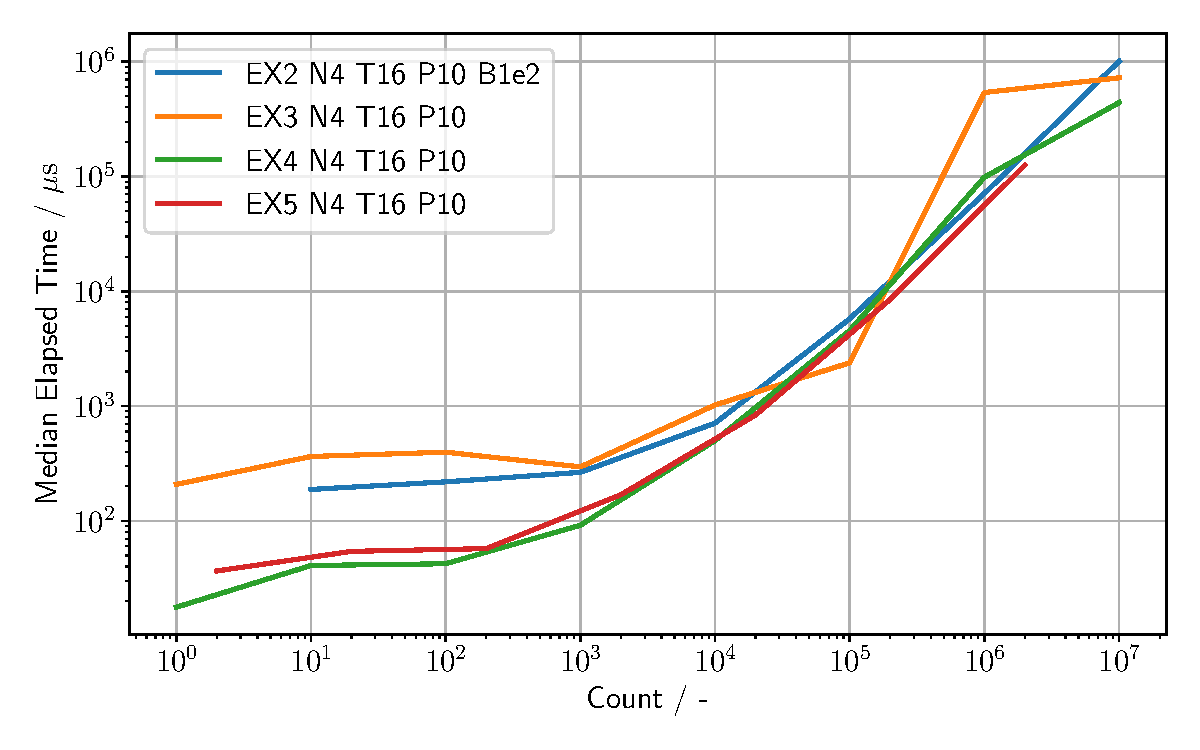
\includegraphics[width=0.9\linewidth]{figures/Ex5_3.pdf}
        \caption{Median elapsed time for 4 nodes, 16 tasks per node and powers of 10, for algorithms from the 
        previous exercises. There is no major difference in the performance of \fun{MY\_Reduce\_T()} + \fun{MY\_Bcast()} 
        compared to \fun{MY\_Allreduce\_T}. For count $< 10^{4}$, \fun{MY\_Reduce\_T()} + \fun{MY\_Bcast()} 
        is of sligthly better performance, but for larger count \fun{MY\_Allreduce\_T} is more efficient. 
        Additionally, we can see that for even higher count, the implementatation of exercise 3 -- \fun{MY\_Allreduce\_T()}
        -- seems to outperform \fun{MY\_Reduce\_T()} + \fun{MY\_Bcast()} and \fun{MY\_Allreduce\_T}.}
        \label{Ex5_3_p}
    \end{center}
\end{figure}

\pagebreak

In figures \ref{Ex5_1_p} and \ref{Ex5_2_p} below we can observe that the \fun{MY\_Allreduce\_T()} tree algorithm 
benefits from a low number of tasks per processes. Interestingly, the timings for powers of 2 in figure \ref{Ex5_2_p}
seem to all reduce their slope again when the blocksize adjustment occurs, while the timings for powers 10 in figure
\ref{Ex5_1_p} on the right do not.

\begin{figure}[h]
\centering
    \begin{minipage}[t]{.49\textwidth}
        \centering
        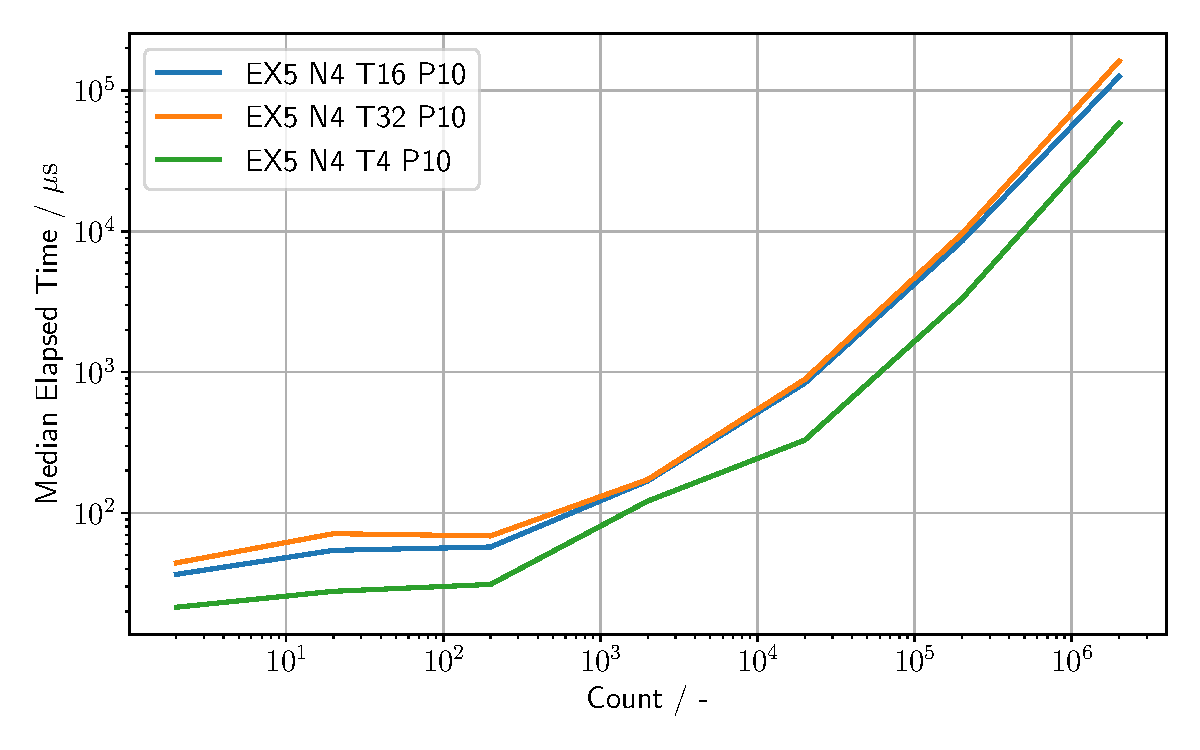
\includegraphics[width=1.0\linewidth]{figures/Ex5_1.pdf}
        \captionof{figure}{\fun{MY\_Allreduce\_T()} tree algorithm with 4 
        nodes and powers of 2.}
        \label{Ex5_1_p}
    \end{minipage}%
    \hfill
    \begin{minipage}[t]{.49\textwidth}
        \centering
        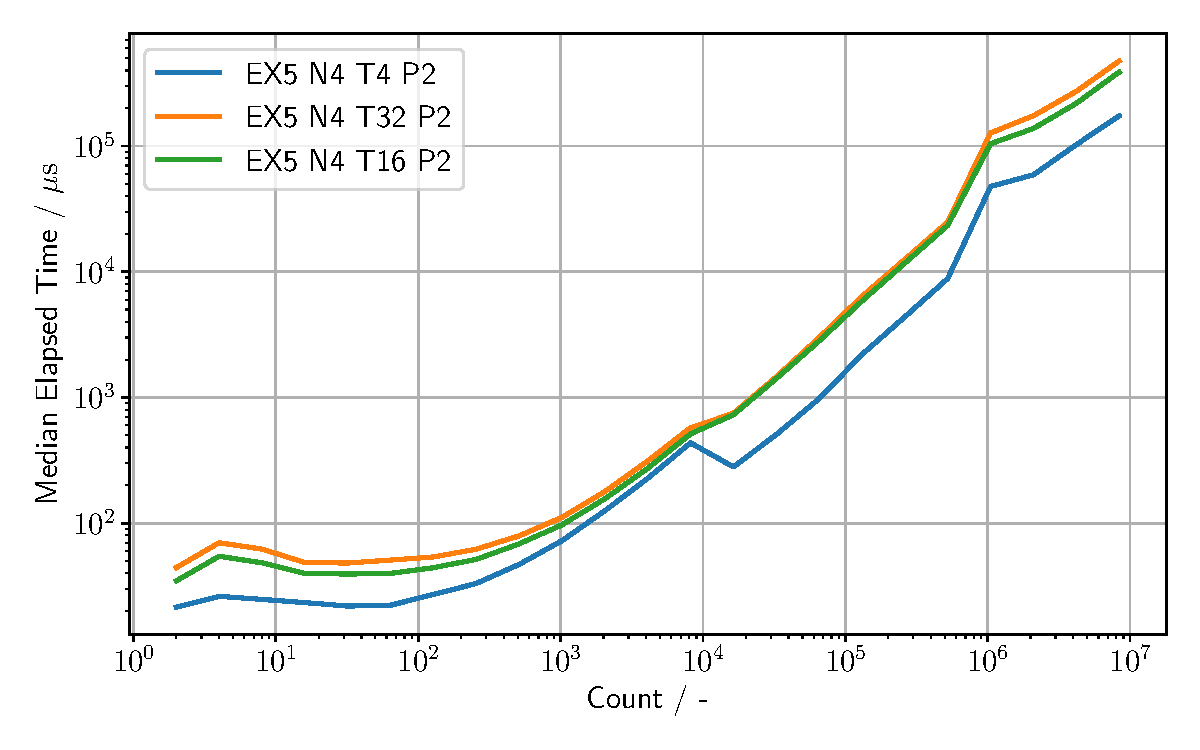
\includegraphics[width=1.0\linewidth]{figures/Ex5_2.pdf}
        \captionof{figure}{\fun{MY\_Allreduce\_T()} tree algorithm with 4 
        nodes and powers of 10. Visible slope reduction due to blocksize adjustment 
        at count = $10^6$ again.}
        \label{Ex5_2_p}
    \end{minipage}
\end{figure}


